% vim: set ts=4 expandtab sw=4 foldmethod=marker: 
\documentclass[11pt]{beamer}
\usetheme{CambridgeUS}

%|--- Packages and Configs {{{1
\usepackage[utf8]{inputenc}
\usepackage[T1]{fontenc}    
\usepackage[brazil]{babel}

\usepackage{amsmath}
\usepackage{amsfonts}
\usepackage{amssymb}
\usepackage{amsthm}
\usepackage{mathrsfs}

\usepackage{bm}

\usepackage{hyperref}
\usepackage{enumerate}

\usepackage{subfiles}


%%% allows you to insert many figures indexed by (a), (b), ... on a figure environment
\usepackage{float} 
\usepackage[caption = false]{subfig}

\usepackage{tikz}
\usetikzlibrary{matrix,positioning}

\usepackage{pgfplots}
\pgfplotsset{compat=1.17}

\usetikzlibrary{fadings}
\tikzfading[name=fade out, inner color=transparent!0, outer color=transparent!100]

\usetikzlibrary{shadings}
\definecolor{azulClaro}{RGB}{65,105,225}

\usepackage{ifthen} %% gives if conditionals when using newcommand

% 1}}}

%%%%%%%%%%%%%%%%%  Math operators %%%%%%%%%%%%%%%%%%%%%%%
%%% {{{1
\DeclareMathOperator {\card}{card}
\DeclareMathOperator {\LI}{L.I.}
\DeclareMathOperator {\Id}{\mathbbm{1}}
\DeclareMathOperator {\Diag}{Diag}
\DeclareMathOperator {\Diagrama}{Dgm}
\DeclareMathOperator {\iid}{i.i.d}
\DeclareMathOperator {\prob}{\mathbb{P}}
\DeclareMathOperator {\birth}{birth}
\DeclareMathOperator {\death}{death}
\DeclareMathOperator {\Rad}{Rad}

\DeclareMathOperator {\ber}{Bernoulli}
\DeclareMathOperator {\sgn}{sgn}

\DeclareMathOperator*{\argmin}{arg\,min}
\DeclareMathOperator{\Erro}{Erro}

\DeclareMathOperator{\R}{\mathbb{R}}
\DeclareMathOperator{\Q}{\mathbb{Q}}
\DeclareMathOperator{\Z}{\mathbb{Z}}
\DeclareMathOperator{\N}{\mathbb{N}}


\DeclareTextFontCommand{\emph}{\bfseries\em} %% redefining \emph{} with bold and italic font
\DeclareMathOperator{\definedAs}{\vcentcolon = }

\DeclareMathOperator {\Imagem}{ Im }

\DeclareMathOperator {\AMod}{ \operatorname{ \mathbf{A-Mod} }}
\DeclareMathOperator {\Set}{ \mathbf{Set} }
\DeclareMathOperator {\Vect}{ \mathbf{Vect}_{\mathbb{K}} }
%%% 1}}}
%%%%%%%%%%%%%%%%%%%%%%%%%%%%%%%%%%%%%%%%%%%%%%%%%%%%%%%%%

%|--- Begin Document {{{1
\begin{document}

%%%%%%%% INTRO

    % frame 1 {{{2 
    \begin{frame}
        \frametitle{Introdução}

        Estes slides consistem em apresentar meus resultados
        preliminares para os seguintes problemas

        \begin{enumerate}
            \item \textbf{Primeiro Problema}:
            \begin{center}
                    \emph{
                        Estudar \textbf{``propriedades persistentes''} de uma
                        coleção de pontos oriundos de um Processo
                        Pontual não estacionário;
                    }
            \end{center}

        \item \textbf{Segundo Problema}:
            \begin{center}
                \begin{itemize}
                    \item
                        \emph{
                            Avaliar o comportamento de um grafo de conversas
                            referentes a COVID-19 no Twitter
                        }
                    \item
                        \emph{ e estudar as
                            \textbf{``propriedades persistentes''} de seu subgrafo formado
                            pelas mensagens classificadas como Fake News;
                        }
                \end{itemize}
            \end{center}
        \end{enumerate}
    \end{frame}
    % END frame1 2}}}

    % frame2 {{{2 
    \begin{frame}
        \frametitle{Introdução}
        \begin{itemize}
            \item
                O termo \textbf{``propriedades persistentes''} 
                é destacado de propósito;

            \item 
                De fato, este termo vem por causa da \textbf{Homologia
                Persistente};

            \item 
                E será objeto central de toda minha argumentação;

            \item Para isso, antes de prosseguirmos 

            \item Precisamos entendê-la

            \item E criar intuição sobre a ferramenta central para nosso
                trabalho...
        \end{itemize}
    \end{frame}
    % END frame2 2}}}

    % frame 3 {{{2 
    \begin{frame}
        \frametitle{O que é Homologia Persistente}
        \begin{itemize}
            \item 
                Como dito no slide anterior

            \item 
                Por \textbf{propriedades persistente} nos referimos
                a todo e qualquer elemento do ramo da
                \begin{center}
                    \textbf{Homologia Persistente}
                \end{center}

            \item 
                Ramo este que se fundamenta fortemente na
                \textbf{Homologia Simplicial} \\[1cm]
                \begin{tikzpicture}[yscale=0.4, xscale=0.6]
                    \draw(0,0) node[left, scale=1.4] {Hom. Simplicial};
                    \draw(4,0) node[right, scale=1.4] {Hom. Persistente};

                    \draw[-, line width=2pt] 
                        (0,1) -- (0,-1) --(3,-1) -- (3,-2) -- (4,0) -- 
                        (3,2) -- (3, 1) -- (0,1);
                              
                \end{tikzpicture}

        \end{itemize}
    \end{frame}
    % END frame 2}}}

    % frame 4 {{{2 
    \begin{frame}
        \frametitle{O que é Homologia Persistente}
        \framesubtitle{A Homologia Simplicial}

        \begin{itemize}
            \item
                Com um olhar mais ingênuo

            \item 
                Para desenvolvermos intuição

            \item
                Pensaremos na \textbf{Homologia Simplicial}
                como 
                \begin{itemize}
                    \item
                        uma ferramenta capaz de detectar
                        \textit{certas propriedades geométricas}
                        de um conjunto

                    \item 
                        Tais Propriedades Geométricas serão:
                        \begin{center}
                            componentes conexas ou ``buracos''
                        \end{center}
                \end{itemize}
        \end{itemize}

        \begin{tikzpicture}
            % coffee {{{3

            % Saucer
            \begin{scope}[shift={(0,-1)}]
                \fill [black!87.5, path fading=fade out]
                  (0,-2/8) ellipse [x radius=6/4, y radius=3/4];
                \shade [left color=gray!20, right color=gray!80]
                  (0,0) ++(180:1.25) arc (180:360:5/4 and 5/8+1/16);
                \shade [left color=gray!40, right color=gray!20]
                  (0,0) ellipse [x radius=5/4, y radius=5/8];
                \shade [right color=gray!40, left color=gray!20]
                  (0,0) ellipse [x radius=5/4/2, y radius=5/8/2];
                \shade [left color=gray!40, right color=gray!20]
                  (0,-1/16) ellipse [x radius=5/4/2-1/16, y radius=5/8/2-1/16];
            \end{scope}

            % Handle
            \begin{scope}[shift=(10:7/8), rotate=-30, yslant=1/2, xslant=-1/8]
              \shade [top color=gray!80, bottom color=gray!30]
                (0,0) arc (130:-100:3/8 and 1/2) -- ++(0,1/4) arc (-100:130:1/8 and 1/4) -- cycle;
              \shade [top color=gray!10, bottom color=gray!60]
                (0,0) arc (130:-100:3/8 and 1/2) -- ++(0,1/32) arc (-100:130:1/4 and 1/3) -- cycle;
            \end{scope}

            % Cup
            \fill [black!75, path fading=fade out]
                (0,-1) ellipse [x radius=3/4, y radius=1/2];
            \shade [left color=gray!60, right color=gray!30]
              (-1,0) arc (180:360:1 and 5/4);
            \shade [bottom color=gray, top color=gray!30, opacity=1/2]
              (-1,0) arc (180:360:1 and 5/4);
            \shade [left color=gray!20, right color=gray!40]
              (0,0) ellipse [x radius=1, y radius=1/2];
            \shade [left color=gray!40, right color=gray!20]
              (0,0) ellipse [x radius=1-1/16, y radius=1/2-1/16];
            \shade [bottom color=gray, top color=gray!10, opacity=1/2]
              (0,0) ellipse [x radius=1-1/16, y radius=1/2-1/16];

            % Coffee
            \begin{scope}
            \clip ellipse [x radius=1-1/16, y radius=1/2-1/16];
            \fill [brown!25!black]
              (0,-1/4) ellipse [x radius=3/4, y radius=3/8];
            \fill [brown!50!black, path fading=fade out]
              (0,-1/4) ellipse [x radius=3/4, y radius=3/8];
            \end{scope}

            \begin{scope}[shift={(0,0.2)}]
                \draw[color=gray, line width=5pt] (0,0) ..controls (-0.3,0.3) and (0.3,0.6) .. (0,0.9);
            \end{scope}
            \begin{scope}[shift={(0.2,0.2)}]
                \draw[color=gray, line width=5pt] (0,0) ..controls (-0.3,0.3) and (0.3,0.6) .. (0,0.9);
            \end{scope}
            \begin{scope}[shift={(-0.2,0.2)}]
                \draw[color=gray, line width=5pt] (0,0) ..controls (-0.3,0.3) and (0.3,0.6) .. (0,0.9);
            \end{scope}
            % coffee 3}}}

            % toro {{{3
            \begin{scope}[xscale=6/6, yscale=1/6, shift={(5,0)}]
                \foreach \angle in {90, 89, ..., -90}{
                    
                    \pgfmathsetmacro\x{ cos(\angle)  }
                    \pgfmathsetmacro\y{ 2.3*sin(\angle)  }
                    \pgfmathsetmacro\intensidadeB{ max(90*cos(\angle/0.8), 49)  }
                    \pgfmathsetmacro\intensidadeA{ 100 - max(80*cos(\angle/0.85),10 )  }

                    \fill[azulClaro!\intensidadeA!black!\intensidadeB]
                        (\x,\y) ellipse (0.5cm and 2.1cm);

                    \fill[azulClaro!\intensidadeA!black!\intensidadeB]
                        (-\x,\y) ellipse (0.5cm and 2.1cm);
                }

                \pgfmathsetmacro\x{ cos(90)  }
                \pgfmathsetmacro\y{ 2.3*sin(-90)  }
                \pgfmathsetmacro\intensidadeB{ max(90*cos(-90/0.8), 49)  }
                \pgfmathsetmacro\intensidadeA{ 100 - max(80*cos(-90/0.85),10 )  }
                                                    
                \shade[
                    shading=ball,
                    outer color = azulClaro!\intensidadeA!black!\intensidadeB,
                    inner color = azulClaro!20
                ]
                    (\x,\y) ellipse (0.5 cm and 2.1cm);
            \end{scope}
            % 3}}}

            % papel {{{3
            \begin{scope}[scale=1/6, shift={(35,0)}]
            \def\mySquare{(14,-4) rectangle (26, 4.5)}

            \draw[very thick, line width = 1pt] \mySquare;
            \begin{scope}[even odd rule]
                \clip \mySquare;
                \foreach \x in {0,1, ..., 26}{
                        \draw (\x,-4) -- + (10,10);
                }
            \end{scope}
            
            \draw (20,-6) node {$[0,2\pi] \times [0,2\pi]$};1

            \draw[->, thick, line width=1pt] (14,-4) -- (20,-4);
            \draw[->, thick, line width=1pt] (14,4.5) -- (20,4.5);
            \draw[->, thick, line width=1pt] (14,-4) -- (14,0.2);
            \draw[->, thick, line width=1pt] (26,-4) -- (26,0.2);
            \end{scope}
            % 3}}}

        \end{tikzpicture}

    \end{frame}
    % END frame 2}}}

    % frame 5 {{{2 
    \begin{frame}
        \frametitle{O que é a Homologia Persistente}
        \framesubtitle{Motivação}

        \begin{itemize}

            \item
                Técnicas de análise estatística baseiam-se
                quase certamente em 
                \begin{itemize}
                    \item 
                        Ajustar um hiperplano a uma amostra

                    \item 
                        Seguindo certos critérios de minimização 
                \end{itemize}
        \end{itemize}
        % figura {{{3
        \begin{figure}[h]
            \centering
            \subfloat[Valores da amostra de 50 indivíduos.]{
            %% drawing \\beginVimFold
            \begin{tikzpicture}[scale=0.6]
                \begin{axis}[
                    xmin = 130, xmax = 420,
                    ymin = 51,  ymax = 159,
                    xtick distance = 50,
                    ytick distance = 10,
                    xlabel=Colesterol Total,
                    ylabel = Level de Glicose (mg/dL),
                    %legend style = {at = {(0.65,1)}},
                    legend pos = north east,
                ]
                \addplot[ only marks, color = red, mark = 10-pointed star ]
                    table [x index = 0, y index = 1, col sep = comma]
                    {dados/totChol_glucose_CHD0.csv};

                \addplot[only marks, color = blue, mark = *]
                    table [x index = 0, y index = 1, col sep = comma]
                    {dados/totChol_glucose_CHD1.csv};
                \end{axis}
            \end{tikzpicture}
            %% \\endVimFold
            } 
            \subfloat[Exemplo de hiperplano separando os pontos.]{
            %% drawing \\beginVimFold
            \begin{tikzpicture}[scale=0.6]
                \begin{axis}[
                    xmin = 130, xmax = 420,
                    ymin = 51,  ymax = 159,
                    xtick distance = 50,
                    ytick distance = 10,
                    xlabel=Colesterol Total,
                    ylabel = Level de Glicose (mg/dL),
                    %legend style = {at = {(0.65,1)}},
                    legend pos = north east,
                ]
                \addplot[only marks, color = red, mark = 10-pointed star]
                    table [x index = 0, y index = 1, col sep = comma]
                    {dados/totChol_glucose_CHD0.csv};

                \addplot[only marks, color = blue, mark = *]
                    table [x index = 0, y index = 1, col sep = comma]
                    {dados/totChol_glucose_CHD1.csv};

                \addplot[domain = 130:350, color = black, dashed]  
                    { -(60.0/150.0) * (x - 150.0) + 110.0};

                \draw[thick, ->]
                    (axis cs: 150,110) -- (axis cs: 160,114)
                    node[above] {$\hat{w}$};
                \end{axis}

            \end{tikzpicture}
            %% \\endVimFold
            } 
        \end{figure}
        % END figura 3}}}

    \end{frame}
    % END frame 2}}}

    % frame 6 {{{2 
    \begin{frame}
        \frametitle{O que é a Homologia Persistente}
        \framesubtitle{Motivação}

        \begin{itemize}
            \item
                Lado negativo destas técnicas:
                \begin{enumerate}
                    \item
                        Propriedades locais da amostra são perdidos
                    \item
                        Em prol de se resolver um problema de minimização
                \end{enumerate}

            \item
                Observe-se como os pontos azuis estão mais distantes entre si;

            \item 
                Se comparados aos pontos vermelhos;
        \end{itemize}

        % figura {{{3
        \begin{figure}[h]
            \centering
            \begin{tikzpicture}[scale=0.6]
                \begin{axis}[
                    xmin = 130, xmax = 420,
                    ymin = 51,  ymax = 159,
                    xtick distance = 50,
                    ytick distance = 10,
                    xlabel=Colesterol Total,
                    ylabel = Level de Glicose (mg/dL),
                    %legend style = {at = {(0.65,1)}},
                    legend pos = north east,
                ]
                \addplot[ only marks, color = red, mark = 10-pointed star ]
                    table [x index = 0, y index = 1, col sep = comma]
                    {dados/totChol_glucose_CHD0.csv};

                \addplot[only marks, color = blue, mark = *]
                    table [x index = 0, y index = 1, col sep = comma]
                    {dados/totChol_glucose_CHD1.csv};
                \end{axis}
            \end{tikzpicture}
        \end{figure}
        % END figura 3}}}

    \end{frame}
    % END frame 2}}}

    % frame 7 {{{2 
    \begin{frame}
        \frametitle{O que é a Homologia Persistente}
        \framesubtitle{Motivação}

        \begin{itemize}

            \item
                \textbf{Observações} \\[0.4cm]
                \begin{itemize}
                    \item
                        Seria legal incorporar propriedades locais
                        no modelo de análise\\[0.2cm]

                    \item
                        E também seria legal avaliar as características
                        geométricas da amostra\\[0.4cm]

                \end{itemize}

            \item
                Motivados por estes pontos,
                as seguintes ideais parecem razoáveis \\[0.4cm]
                \begin{enumerate}
                    \item
                        Agrupar os pontos distantes entre si, $d(x,y) \leq r$\\[0.2cm]

                    \item
                        E aplicar a homologia simplicial nestes agrupamentos (simplexos)
                \end{enumerate}
        \end{itemize}


    \end{frame}
    % END frame 2}}}

    % frame 8 {{{2 
    \begin{frame}
        \frametitle{O que é a Homologia Persistente}
        \framesubtitle{Motivação}

        % figura {{{3
        \begin{figure}[h]
            \centering
            \subfloat[]{
            %% drawing \\beginVimFold
            \begin{tikzpicture}[scale=0.6]
                \begin{axis}[
                    xmin = 120, xmax = 430,
                    ymin = 41,  ymax = 149,
                    xtick distance = 50,
                    ytick distance = 10,
                    xlabel=Colesterol Total,
                    ylabel = Level de Glicose (mg/dL),
                    %legend style = {at = {(0.65,1)}},
                    legend pos = north east,
                ]
                \addplot[only marks, color = red, mark = 10-pointed star]
                    table [x index = 0, y index = 1, col sep = comma]
                    {dados/totChol_glucose_CHD0.csv};
                \addlegendentry{\footnotesize CHD10 = 0}

                \addplot[only marks, color = red, mark = *, mark size = 0.325cm, opacity = 0.2]
                    table [x index = 0, y index = 1, col sep = comma]
                    {dados/totChol_glucose_CHD0.csv};

                \end{axis}

            \end{tikzpicture}
            %% \\endVimFold
            }
            \subfloat[]{
            %% drawing \\beginVimFold
            \begin{tikzpicture}[scale=0.6]
                \begin{axis}[
                    xmin = 120, xmax = 430,
                    ymin = 41,  ymax = 149,
                    xtick distance = 50,
                    ytick distance = 10,
                    xlabel=Colesterol Total,
                    ylabel = Level de Glicose (mg/dL),
                    legend pos = north east,
                ]
                \addplot[only marks, color = red, mark = 10-pointed star]
                    table [x index = 0, y index = 1, col sep = comma]
                    {dados/totChol_glucose_CHD0.csv};
                \addlegendentry{\footnotesize CHD10 = 0}

                \addplot[only marks, color = red, mark = *, mark size = 0.325cm, opacity = 0.2]
                    table [x index = 0, y index = 1, col sep = comma]
                    {dados/totChol_glucose_CHD0.csv};

                \addplot[black, quiver={u=\thisrow{u},v=\thisrow{v}}, -, thick]
                table[row sep =\\] {
                    % \\beginVimFold
                    x y u v
                    224 68 1 5 \\
                    224 68 17 6 \\
                    224 68 -9 -7 \\
                    224 68 14 5 \\
                    224 68 -5 5 \\
                    224 68 -11 7 \\
                    224 68 5 5 \\
                    224 68 16 -8 \\
                    224 68 -14 9 \\
                    224 68 -24 4 \\
                    199 76 18 8 \\
                    199 76 26 -3 \\
                    199 76 -5 12 \\
                    199 76 20 -3 \\
                    199 76 14 -1 \\
                    199 76 -20 1 \\
                    199 76 -11 -8 \\
                    199 76 11 1 \\
                    199 76 1 -4 \\
                    199 76 -26 -1 \\
                    290 87 5 -12 \\
                    217 84 21 4 \\
                    217 84 8 -11 \\
                    217 84 -23 4 \\
                    217 84 2 -11 \\
                    217 84 -4 -9 \\
                    217 84 12 -11 \\
                    217 84 -7 -7 \\
                    165 87 16 -1 \\
                    165 87 -12 -5 \\
                    165 87 29 1 \\
                    165 87 14 -10 \\
                    165 87 -2 3 \\
                    181 86 13 2 \\
                    181 86 -2 -9 \\
                    181 86 -8 -11 \\
                    181 86 -18 4 \\
                    238 88 16 2 \\
                    238 88 13 -4 \\
                    225 73 16 1 \\
                    225 73 13 0 \\
                    225 73 -6 0 \\
                    225 73 -12 2 \\
                    225 73 4 0 \\
                    225 73 -15 4 \\
                    225 73 -25 -1 \\
                    254 90 -3 -6 \\
                    241 74 -3 -1 \\
                    241 74 10 10 \\
                    241 74 -22 -1 \\
                    241 74 23 -4 \\
                    241 74 -28 1 \\
                    241 74 -12 -1 
                    241 74 17 1 \\
                    153 82 26 -5 \\
                    153 82 20 -7 \\
                    153 82 10 8 \\
                    215 61 4 12 \\
                    215 61 25 -1 \\
                    238 73 13 11 \\
                    238 73 -19 0 \\
                    238 73 26 -3 \\
                    238 73 -25 2 \\
                    238 73 -9 0 \\
                    238 73 20 2 \\
                    251 84 7 -9 \\
                    283 68 -3 -3 \\
                    283 68 -19 2 \\
                    283 68 17 7 \\
                    283 68 12 7 \\
                    280 65 -16 5 \\
                    280 65 15 10 \\
                    219 73 -6 2 \\
                    219 73 10 0 \\
                    219 73 -9 4 \\
                    219 73 -19 -1 \\
                    264 70 -6 5 \\
                    337 77 -22 -7 \\
                    213 75 16 -2 \\
                    213 75 -3 2 \\
                    213 75 -13 -3 \\
                    300 75 -5 0 \\
                    300 75 15 -5 \\
                    179 77 9 -9 \\
                    179 77 21 -5 \\
                    179 77 -6 -2 \\
                    229 73 29 2 \\
                    229 73 -19 4 \\
                    229 73 -29 -1 \\
                    188 68 12 4 \\
                    188 68 -15 7 \\
                    210 77 -10 -5 \\
                    200 72 -27 3 \\
                    410 83 -19 -5 \\
                    295 75 20 -5 \\
                    %% \\endVimFold
                };
                \end{axis}

                % correcao de escala no grafico
                % Eixo x =>  1.1cm  = 50
                % Eixo y =>  0.53cm  = 10mg/dL
            \end{tikzpicture}
            %% \\endVimFold
            }
        \end{figure}
        % END figura 3}}}


    \end{frame}
    % END frame 2}}}

    % frame 9 {{{2 
    \begin{frame}
        \frametitle{O que é a Homologia Persistente}
        \framesubtitle{Motivação}

        % figura {{{3
        \begin{figure}[h]
            \centering
            \subfloat[]{
            %% drawing \\beginVimFold
            \begin{tikzpicture}[scale=0.6]
                \begin{axis}[
                    xmin = 120, xmax = 430,
                    ymin = 41,  ymax = 149,
                    xtick distance = 50,
                    ytick distance = 10,
                    xlabel=Colesterol Total,
                    ylabel = Level de Glicose (mg/dL),
                    %legend style = {at = {(0.65,1)}},
                    legend pos = north east,
                ]
                \addplot[only marks, color = blue, mark = *] 
                    table [x index = 0, y index = 1, col sep = comma]
                    {dados/totChol_glucose_CHD1.csv};
                \addlegendentry{\footnotesize risco de doença arterial coronária = 1}

                \addplot[only marks, color = blue, mark = *, mark size = 0.325cm, opacity = 0.2] 
                    table [x index = 0, y index = 1, col sep = comma]
                    {dados/totChol_glucose_CHD1.csv};
                \end{axis}

            \end{tikzpicture}
            %% \\endVimFold
            }
            \subfloat[]{
            %% drawing \\beginVimFold
            \begin{tikzpicture}[scale=0.6]
                \begin{axis}[
                    xmin = 120, xmax = 430,
                    ymin = 41,  ymax = 149,
                    xtick distance = 50,
                    ytick distance = 10,
                    xlabel=Colesterol Total,
                    ylabel = Level de Glicose (mg/dL),
                    %legend style = {at = {(0.65,1)}},
                    legend pos = north east,
                ]
                \addplot[only marks, color = blue, mark = *]
                    table [x index = 0, y index = 1, col sep = comma]
                    {dados/totChol_glucose_CHD1.csv};
                \addlegendentry{\footnotesize risco de doença arterial coronária = 1}

                \addplot[only marks, color = blue, mark = *, mark size = 0.325cm, opacity = 0.2]
                    table [x index = 0, y index = 1, col sep = comma]
                    {dados/totChol_glucose_CHD1.csv};

                \addplot[black, quiver={u=\thisrow{u},v=\thisrow{v}}, -, thick]
                table[row sep =\\] {
                    % \\beginVimFold
                    x y u v
                    253 70 7 2 \\
                    253 70 -17 -3 \\
                    253 70 5 5 \\
                    260 72 -24 -5 \\
                    260 72 -2 3 \\
                    236 67 22 8 \\
                    334 77 -7 -5 \\
                    %% \\endVimFold
                };

                \end{axis}

                % correcao de escala no grafico
                % Eixo x =>  1.1cm  = 50
                % Eixo y =>  0.53cm = 10mg/dL

            \end{tikzpicture}
            %% \\endVimFold
            }
        \end{figure}
        % END figura 3}}}

    \end{frame}
    % END frame 2}}}

    % frame 10 {{{2 
    \begin{frame}
        \frametitle{O que é a Homologia Persistente}
        \framesubtitle{Motivação}

        \begin{itemize}
            \item
                Até agora tudo bem...

            \item
                Porém:

                \begin{center}
                    Qual valor $r$ usar para agrupar os pontos em função
                    de suas distâncias $d(x,y) \leq r$???
                \end{center}

            \item
                Aí que surge a 
                \[
                \begin{tikzpicture}
                    \draw[fill=blue!20!white, opacity=0.8]
                        (0,0) ellipse (3cm and 1cm) node[midway, scale=1.2] 
                        {\textbf{Homologia Persistente}};
                \end{tikzpicture}
                \]

        \end{itemize}

    \end{frame}
    % END frame 2}}}

    % frame 11 {{{2 
    \begin{frame}
        \frametitle{O que é a Homologia Persistente}
        \framesubtitle{Finalmente, a Homologia Persistente}

        %\textbf{Definição da Homologia Persistente}
        \begin{itemize}
            \item
                Seja $X$ um conjunto finito (a amostra);

            \item
                E $X_r$ uma sequência indexada por $r \in \R_{\geq 0}$:
                \begin{equation*}
                    X_r = \{\sigma \subseteq X; x,y \in d(x,y) \leq r\}
                \end{equation*}

            \item Onde 
                \begin{equation*}
                    X_0 \subseteq X_1 \subseteq X_2 \subseteq \cdots
                \end{equation*}

            \item
                $\{X_r\}_{r \in \R_{\geq 0}}$ será chamado de filtração

            \item 
                Temos o diagrama dos grupos de homologia para cada $X_r$:
        \end{itemize}
        
    \end{frame}
    % END frame 2}}}

    % frame 12 {{{2 
    \begin{frame}
        \frametitle{O que é a Homologia Persistente}
        \framesubtitle{Finalmente, a Homologia Persistente}
        \subfile{pics/diagrama_hom_persistente.tex}
    \end{frame}
    % END frame 2}}}
    
%%%%%%%% Convergencia do numero de Betti


%%%%%%%%%% Twitter
%	% frame 1 {{{2
%	\begin{frame}
%		\frametitle{O que é um Tweet}
%		\begin{enumerate}
%			\item Um tweet pode ser abstraído como o elemento da Figura abaixo
%			\begin{figure}[h]
%				\centering
%				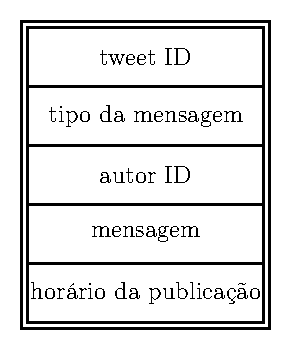
\includegraphics{pics/pic0.pdf}
%			\end{figure}
%			\item \textbf{Tipo da mensagem} pode ser igual a "mensagem", "RT", "resposta", ou "Quote"
%		\end{enumerate}
%		\end{frame}
%	% END frame 1 2}}}
%
%	% frame 2 {{{2
%	\begin{frame}
%		\frametitle{Intereção entre Tweets}
%		\begin{enumerate}
%			\item Tweets podem interagir entre si, por exemplo:
%			\begin{figure}[h]
%				\centering
%				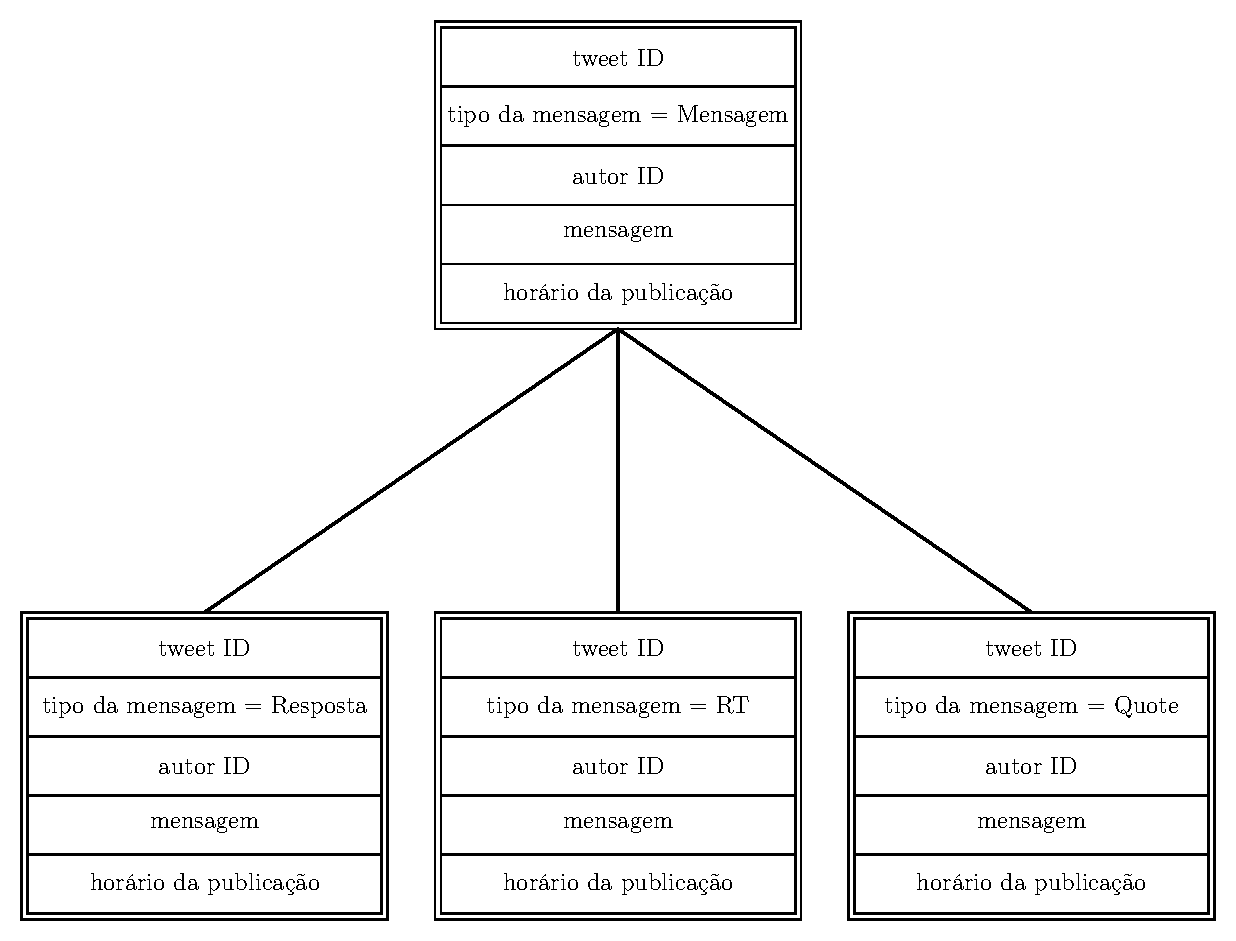
\includegraphics[scale=0.45]{pics/pic1.pdf}
%			\end{figure}
%		\end{enumerate}
%		\end{frame}
%	% END frame 2 2}}}
%
%	% frame 3 {{{2
%	\begin{frame}
%		\frametitle{Intereção entre Tweets}
%		\begin{enumerate}
%			\item A intereçaão entre os tweets pode continuar indefinitivamente.
%			\begin{figure}[h]
%				\centering
%				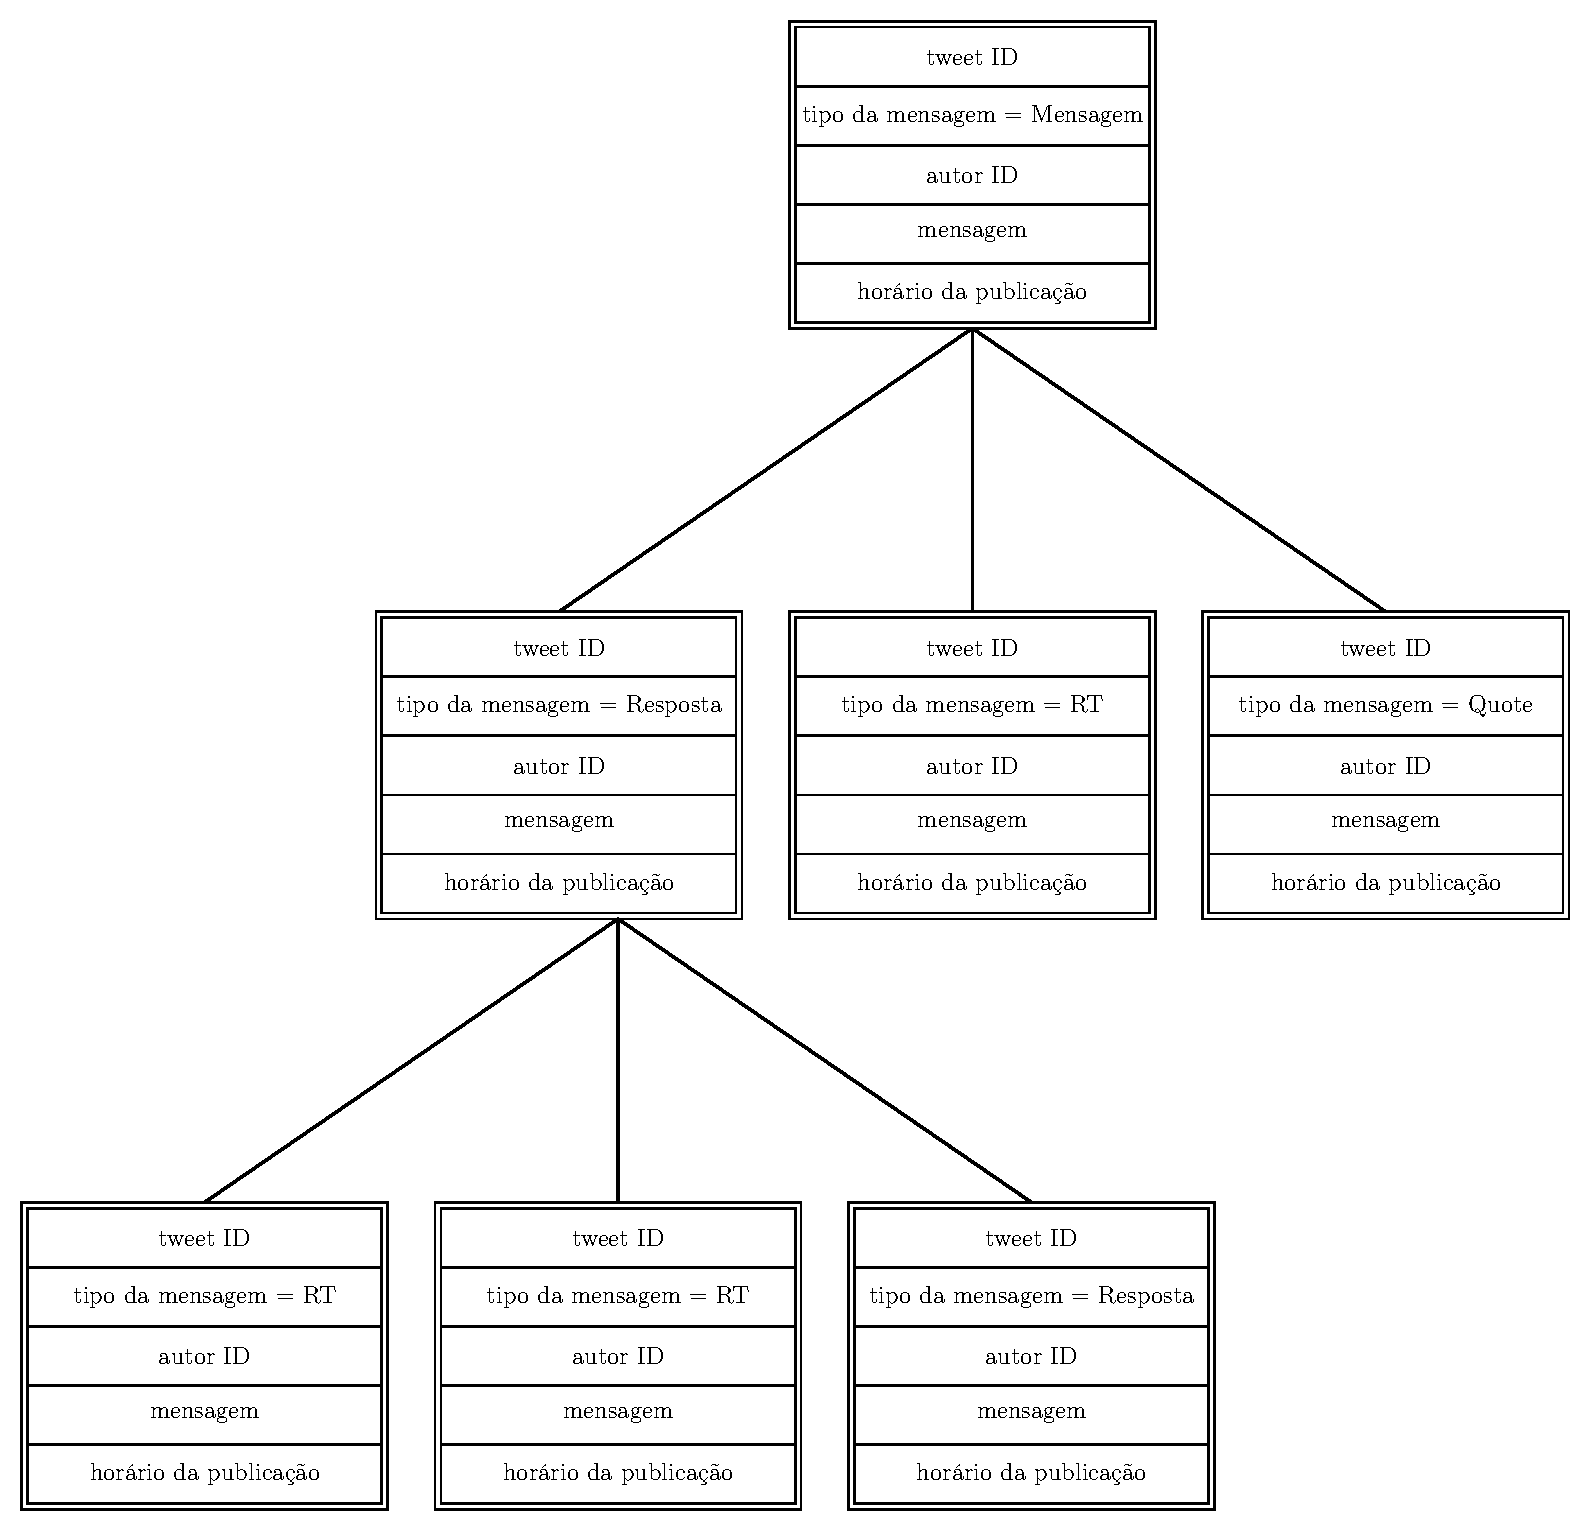
\includegraphics[scale=0.3]{pics/pic2.pdf}
%			\end{figure}
%		\end{enumerate}
%		\end{frame}
%	% END frame 3 2}}}
%
%	% frame 4 {{{2
%	\begin{frame}
%		\frametitle{Grafo formado pelos Tweets}
%		\begin{enumerate}
%			\item Os tweets assim nos fornecem uma sequência de árvores, 
%				que será o objeto de nossa análise;
%			\item \textbf{Obs}: Os IDs dos tweets são únicos;
%			\item \textbf{Obs}: A intereção entre os autores dos tweets ainda
%				não está sendo levada em conta
%			\item \textbf{Obs} Por interação entre os autores me refiro a situação
%				de, por exemplo, uma pessoa X seguir ou não uma pessoa Y.
%				Sendo que X e Y publicaram um tweet
%		\end{enumerate}
%		\end{frame}
%	% END frame 4 2}}}
%
%	% frame 5 {{{2
%	\begin{frame}
%		\frametitle{Dados coletados até agora}
%		\begin{enumerate}
%			\item Os tweets coletados são referentes a mensagems publicadas no
%				dia 25/03/2021 ocorrendo no período das 18h até as 21h (UTC -3)
%				e contendo alguma das seguintes palavras chaves (em pt):
%				\begin{enumerate}
%					\item vacina \textit{ou}
%					\item cloroquina  \textit{ou}
%					\item covid \textit{ou} corona \textit{ou} covid-19 \textit{ou}
%					\item tratamento antecipado \textit{ou} tratamento precoce \textit{ou}
%					\item azitromicina \textit{ou}
%					\item lockdown
%				\end{enumerate}
%			\item \textbf{Obs} Vale notar que toda mensagem publicada no horário 
%				descrito pode ter um "parent tweet", ou seja,
%				a mensagem coletada é uma resposta ou um RT ou uma Quote
%				de outro tweet. Nestes casos, o tweet pai será incluso 
%				em minha análise, mesmo o mesmo tendo sido publicado fora 
%				do horário ou não contendo alguma das palavras chaves acima.
%		\end{enumerate}
%		\end{frame}
%	% END frame 5 2}}}
%
%	% frame 6 {{{2
%	\begin{frame}
%		\frametitle{Visualização do grafo obtido}
%			\begin{figure}[h]
%				\centering
%				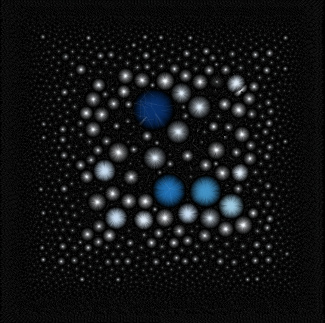
\includegraphics[scale=0.02]{pics/treeGraph_v01_coloured_scaled.png}
%			\end{figure}
%		\end{frame}
%	% END frame 6 2}}}
%
%	% frame 7 {{{2
%	\begin{frame}
%		\frametitle{Algumas mensagens coletadas}
%		\begin{itemize}
%			\item A seguir listo as mensagens que possuim mais de 1000 filhos,
%				i.e., mais de 1000 pessoas interagem com estas mensagens.
%				No total são apenas 7 mensagens.
%		\end{itemize}
%		\end{frame}
%	% END frame 7 2}}}
%
%	% frame 8 {{{2
%	\begin{frame}
%		\frametitle{Algumas mensagens coletadas (mensagens casuais)}
%		\begin{enumerate}
%			\item @leelecarvalho\_ "eu estou fazendo minha parte nesse lockdown, mas não milito em cima
%				de qm ta saindo, pq não sair agora, não anula o fato de eu ter saído antes,
%				tem uns aqui nesse tt mt hipocrita, furou a quarentena toda e agr no lockdown
%				quer pagar de alecrim dourado kkkkk"
%
%			\item @Jouberth19 "lockdown e feriado de 10 dias pra vocês, pq eu vou continuar
%				trabalhando normalmente"
%
%			\item @daycrvg10 "o dia q anunciarem q n há mais covid vai ser O DIA"
%
%			\item @isa\_abrantes10 "Bota a Gabi da FGV nesse governo pra ver se ela não consegue vacina
%				pra todo mundo em uma semana"
%
%		\end{enumerate}
%		\end{frame}
%	% END frame 8 2}}}
%
%	% frame 9 {{{2
%	\begin{frame}
%		\frametitle{Algumas mensagens coletadas (fakenews)}
%		\begin{enumerate}
%
%			\item @bicmuller "vcs tem noção que a Austrália, ZEROU as restrições pra covid ??
%				Sem mascara, bar aberto, estadio de futebol com 100\%
%				de capacidade CABOU COVID NA AUSTRALIA"
%
%			\item @IsabelasemZ "URGENTE - EMPRESÁRIOS  ANUNICAM DOAÇÃO DE 10 MILHÕES  DE VACINAS.
%				Após reunião com Paulo Guedes, os empresários Luciano Hang e Carlos
%				Wizard anunciaram a doação para o SUS de 10 milhões de doses da vacina 
%				contra a Covid.SERÁ QUE A IMPRENSA VAI DIZER QUE ELES SÃO BOLSONARISTAS?"
%
%			\item @BrazilFight "URGENTE: Após reunião com Min. Paulo Guedes, os empresários Luciano Hang
%				e Carlos Wizard anunciaram a doação para o SUS de 10 milhões de doses da 
%				vacina contra a Covid. \#VacinaBrasil https://t.co/pAllXiO6Q6"
%		\end{enumerate}
%		\end{frame}
%	% END frame 9 2}}}
%
%	% frame 11 {{{2
%	\begin{frame}
%		\frametitle{Resultados Preliminares}
%		\begin{itemize}
%			\item Do grafo obtido iremos analisar seu diagrama
%				de persistência de dimensão 0 e 1
%
%			\item Aqui a persistência será obtida pela técnica
%				envolvendo a homologia de caminhos persistentes (path persistent
%				homology)
%			\item Vale notar que para o cálculo desta homologia precisamos
%				ter estabelecido uma matriz de peso para as arestas
%			\item Esta matriz de peso eu adotarei como o intervalo de tempo levado
%				para uma mensagem filha aparecer, em relação ao "parent tweet"
%			\item Com isto obtemos
%		\end{itemize}
%		\end{frame}
%	% END frame 11 2}}}
%
%	% frame 12 {{{2
%	\begin{frame}
%		\frametitle{Resultados Preliminares - dimensão 0}
%			\begin{figure}[h]
%				\centering
%				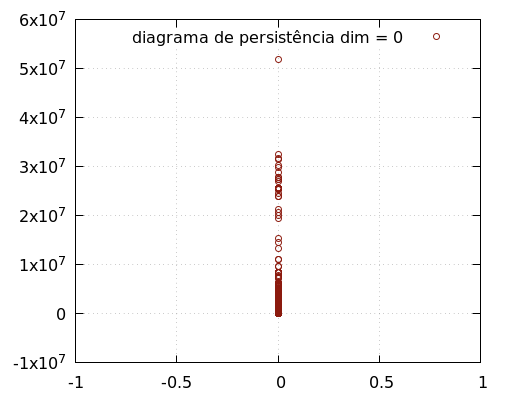
\includegraphics[scale=0.5]{pics/diagram_dim0_v0.png}
%			\end{figure}
%		\end{frame}
%	% END frame 12 2}}}
%
%	% frame 13 {{{2
%	\begin{frame}
%		\frametitle{Resultados Preliminares - dimensão 0}
%			\begin{figure}[h]
%				\centering
%				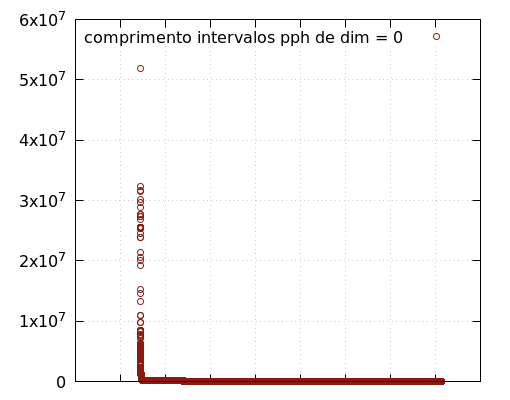
\includegraphics[scale=0.5]{pics/diagram_dim0_v1.png}
%			\end{figure}
%		\end{frame}
%	% END frame 13 2}}}
%
%	% frame 14 {{{2
%	\begin{frame}
%		\frametitle{Resultados Preliminares - dimensão 0}
%			\begin{figure}[h]
%				\centering
%				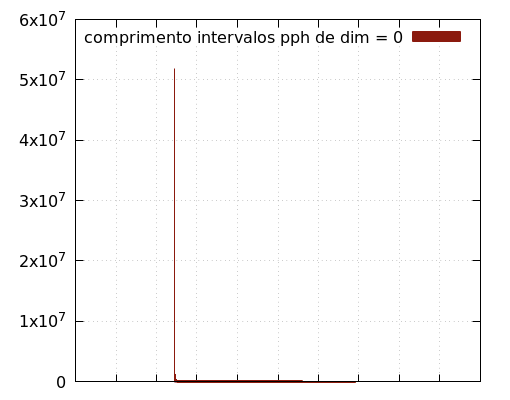
\includegraphics[scale=0.5]{pics/diagram_dim0_v2.png}
%			\end{figure}
%		\end{frame}
%	% END frame 14 2}}}
%
%	% frame 15 {{{2
%	\begin{frame}
%		\frametitle{Resultados Preliminares - dimensão 1}
%			\begin{figure}[h]
%				\centering
%				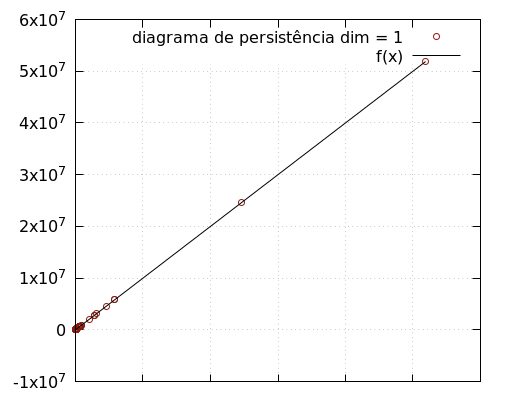
\includegraphics[scale=0.5]{pics/diagram_dim1_v0.png}
%			\end{figure}
%		\end{frame}
%	% END frame 15 2}}}
%
%	% frame 16 {{{2
%	\begin{frame}
%		\frametitle{Resultados Preliminares - dimensão 1}
%			\begin{figure}[h]
%				\centering
%				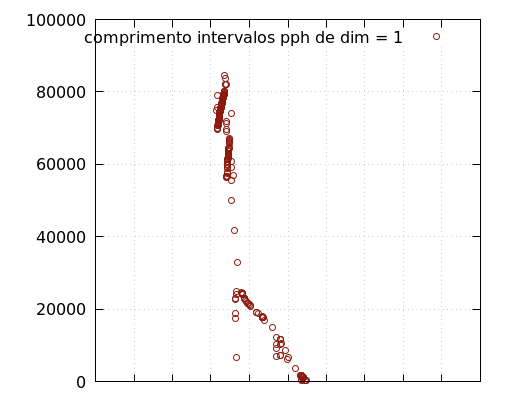
\includegraphics[scale=0.5]{pics/diagram_dim1_v1.png}
%			\end{figure}
%		\end{frame}
%	% END frame 16 2}}}
%
%	% frame 17 {{{2
%	\begin{frame}
%		\frametitle{Resultados Preliminares - dimensão 1}
%			\begin{figure}[h]
%				\centering
%				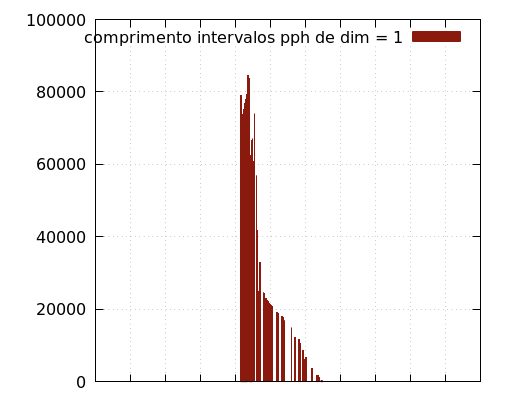
\includegraphics[scale=0.5]{pics/diagram_dim1_v2.png}
%			\end{figure}
%		\end{frame}
%	% END frame 17 2}}}
%
\end{document}
% 1}}}


